\documentclass[
	10pt, % Set the default font size, options include: 8pt, 9pt, 10pt, 11pt, 12pt, 14pt, 17pt, 20pt
	%t, % Uncomment to vertically align all slide content to the top of the slide, rather than the default centered
	aspectratio=169, % Uncomment to set the aspect ratio to a 16:9 ratio which matches the aspect ratio of 1080p and 4K screens and projectors
	% table,
]{beamer}

\graphicspath{{figures/}{./}} % Specifies where to look for included images (trailing slash required)

\input{math_commands.tex}
\usepackage{amsmath}
\usepackage{amsfonts}
\usepackage{booktabs} % Allows the use of \toprule, \midrule and \bottomrule for better rules in tables
\usepackage[textsize=tiny, color=green!30]{todonotes}
\usepackage{tikz}
\usetikzlibrary{
  positioning,
  fit,
  calc,
  shapes,
  arrows.meta,
  shapes.callouts,
  shapes.symbols,
  shapes.geometric,
  shapes.arrows,
  arrows,
  arrows.meta,
  quotes,
  shadows,
  decorations.pathreplacing
}
\usepackage{standalone}
\usepackage{array}
\newcolumntype{L}[1]{>{\raggedright\arraybackslash}p{#1}}

\setuptodonotes{inline, color=yellow!40!white, author=todo}

\usetheme{rpi}
\colorlet{accent}{RPIred}
\renewcommand{\bm}[1]{\symbf{#1}}  % unicode-math compatibility: \symbf replaces \bm
\addbibresource{references.bib}


%----------------------------------------------------------------------------------------
% PRESENTATION INFORMATION
%----------------------------------------------------------------------------------------

\title[Language Model Representations for Efficient Few-Shot Tabular Classification]{Language Model Representations for Efficient Few-Shot Tabular Classification}
% \subtitle{PhD Candidacy Exam}
\author[]{Inwon Kang$^1$, Parikshit Ram, Yi Zhou, Horst Samulowitz, Oshani Seneviratne}
\institute[RPI, IBM]{Rensselaer Polytechcnic Institute$^1$, IBM Research$^2$}

\date[\today]{February 16, 2026}

% Custom macros for paper names
\newcommand{\tdcoler}{\textbf{\texttt{TDColER}}}
\newcommand{\tarl}{\textbf{\textsc{TaRL}}}

% % NOTE: Comment this out if you don't want it
% \AtBeginSection[]{
% 	\begin{frame}[noframenumbering]
% 		\frametitle{Outline}
% 		\begin{columns}[t]
% 			\begin{column}{.05\textwidth}\end{column}
% 			\begin{column}{.45\textwidth}
% 				\tableofcontents[
% 					currentsection,
% 					% sectionstyle=show/hide,
% 					subsectionstyle=hide/show/hide,
% 					sections={-3},
% 				]
% 			\end{column}
% 			\begin{column}{.45\textwidth}
% 				\tableofcontents[
% 					currentsection,
% 					% sectionstyle=show/hide,
% 					subsectionstyle=hide/show/hide,
% 					sections={4-},
% 				]
% 			\end{column}
% 		\end{columns}
% 		% NOTE: If you don't want them to affect the slide number
% 		% \addtocounter{framenumber}{-1}
% 	\end{frame}
% }
%
% % NOTE: Comment this out if you don't want it
% \AtBeginSubsection[]{
% 	\begin{frame}[noframenumbering]
% 		\frametitle{Outline}
% 		\begin{columns}[t]
% 			\begin{column}{.05\textwidth}
% 			\end{column}
% 			\begin{column}{.45\textwidth}
% 				\tableofcontents[
% 					currentsection,
% 					currentsubsection,
% 					% sectionstyle=show/hide,
% 					% subsectionstyle=show/hide,
% 					sections={-3},
% 				]
% 			\end{column}
% 			\begin{column}{.45\textwidth}
% 				\tableofcontents[
% 					currentsection,
% 					currentsubsection,
% 					% sectionstyle=show/hide,
% 					% subsectionstyle=show/hide,
% 					sections={4-},
% 				]
% 			\end{column}
% 		\end{columns}
% 	\end{frame}
% }

\begin{document}
\begin{frame}[plain]
	\titlepage % Output the title slide, automatically created using the text entered in the PRESENTATION INFORMATION block above
\end{frame}

%----------------------------------------------------------------------------------------
% TABLE OF CONTENTS SLIDE
%----------------------------------------------------------------------------------------

% The table of contents outputs the sections and subsections that appear in your presentation, specified with the standard \section and \subsection commands. You may either display all sections and subsections on one slide with \tableofcontents, or display each section at a time on subsequent slides with \tableofcontents[pausesections]. The latter is useful if you want to step through each section and mention what you will discuss.

% \begin{frame}[noframenumbering]
% 	\frametitle{Presentation Overview} % Slide title, remove this command for no title
% 	% NOTE: Two column version
% 	\begin{columns}[t]
% 		\begin{column}{.05\textwidth}
% 		\end{column}
% 		\begin{column}{.45\textwidth}
% 			\tableofcontents[
% 				pausesections,
% 				sections={-3}
% 			]
% 		\end{column}
% 		\begin{column}<+->{.45\textwidth}
% 			\only<.>{\setcounter{tocseccounter}{\slideinframe}}
% 			\advanceslidecounter{-\thetocseccounter}
% 			\tableofcontents[
% 				pausesections,
% 				sections={4-}
% 			]
% 		\end{column}
% 	\end{columns}
% 	% NOTE: One column version
% 	%\tableofcontents[pausesections] % Output the table of contents (break sections up across separate slides)
% \end{frame}

%----------------------------------------------------------------------------------------
% Actual Contents
%----------------------------------------------------------------------------------------

% \begin{frame}
% 	\frametitle{TaRL: Table Representation with Language Model}
% 	\begin{figure}
% 		\centering
% 		\includegraphics[width=\linewidth]{./figures/intro/progression-2.pdf}
% 	\end{figure}
% \end{frame}

\begin{frame}
	\frametitle{Motivation: Few-Shot Tabular Learning}
	\begin{columns}[c]
		\begin{column}{0.55\textwidth}
			\begin{itemize}
				\item New tables constantly arriving with \textbf{few labeled examples}
				\item Traditional ML (XGBoost, Random Forest):
				      \begin{itemize}
					      \item Needs many samples to learn patterns
					      \item Struggles in low-data regimes ($k \leq 32$)
				      \end{itemize}
			\end{itemize}
		\end{column}
		\begin{column}{0.45\textwidth}
			\begin{secondaryblock}{Web Table Applications}
				\begin{itemize}
					\item Product catalogs
					\item Knowledge base exports
					\item Scientific data portals
					\item User-submitted forms
				\end{itemize}
			\end{secondaryblock}
		\end{column}
	\end{columns}
	\vfill
	\heading{Question:} Can LLMs enable \textbf{few-shot learning} on tabular data on the web?
	\begin{itemize}
		\item Web tables have rich semantic content (column names, categorical values)
		\item LLMs contain semantic knowledge from pretraining
	\end{itemize}
\end{frame}

\begin{frame}
	\frametitle{Related Work}
	\begin{itemize}
  \item LLM as classifier (TabLLM~\cite{hegselmannTabLLMFewshotClassification2023}, TabuLa-8B~\cite{gardnerLargeScaleTransfer2024}) 
		      \begin{itemize}
			      \item Requires training
		      \end{itemize}
		\item LLM as feature extractor (\tcite{kasneciEnrichingTabularData2024})
		      \begin{itemize}
			      \item Need to train separate classifier
		      \end{itemize}
        \item Specialized tablular models (TabPFN~\cite{hollmannAccuratePredictionsSmall2025}, ConTextTab~\cite{spinaciConTextTabSemanticsAwareTabular2025})
		      \begin{itemize}
			      \item Not reusable for other modalities
		      \end{itemize}
	\end{itemize}
  \vfill
  \begin{secondaryblock}{Our work}
    We propose a reusable and training-free paradigm for tabular prediction using LLMs
  \end{secondaryblock}
\end{frame}

\begin{frame}{Existing LLM-Based Approaches and Their Costs}
	\heading{Current methods are expensive or require extensive training}
	\vfill
	\begin{columns}[c]
		\begin{column}{0.6\textwidth}
			\heading{Fine-Tuning LLMs }(TabLLM, TabuLa-8B)
			\begin{itemize}
				\item Days of GPU time
				\item Requires labeled data per task
				\item Not practical for new domains
			\end{itemize}
			\vspace{0.5em}
			\heading{Autoregressive Generation }(TabuLa-8B, TabLLM)
			\begin{itemize}
				\item Serialize entire table + prompt
				\item $O(k^2)$ complexity (attention)
			\end{itemize}
			\vspace{0.5em}
			\heading{Specialized Tabular Models }(TabPFN, ConTextTab)
			\begin{itemize}
				\item Table-specific architectures
				\item Only work for tables. Cannot be used for other modalities
			\end{itemize}
		\end{column}
		\begin{column}{0.3\textwidth}
			\vspace{0.5em}
			\begin{center}
				\small
				\begin{tabular}{lc}
					\toprule
					\textbf{Method} & \textbf{Table-Tuning} \\
					\midrule
					TabLLM          & Not reported          \\
					TabPFN          & 2 weeks               \\
					ConTextTab      & 4--10 days            \\
					TabuLa-8B       & 6 days                \\
					\midrule
					\tarl{} (Ours)  & $<$ 1 hour            \\
					\bottomrule
				\end{tabular}
			\end{center}
		\end{column}
	\end{columns}
\end{frame}

\begin{frame}
	\frametitle{Question -- Are LLM Embeddings Useful for Tabular Data?}
	\begin{columns}[c]
		\begin{column}{0.4\textwidth}
			\begin{figure}
				\centering
				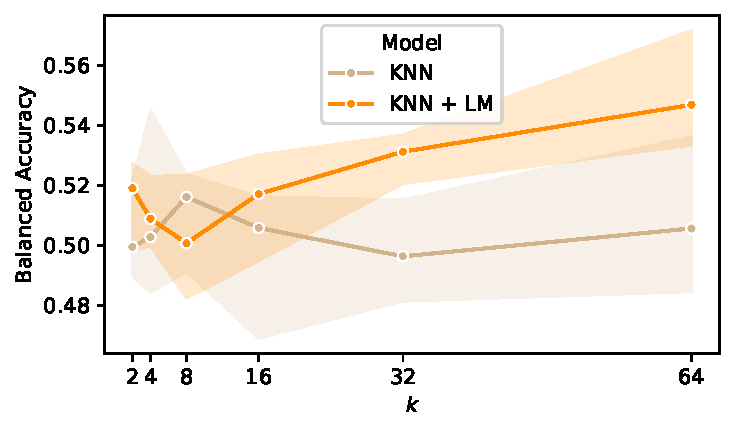
\includegraphics[width=0.9\linewidth]{./figures/carte_cat-knn_embedding.pdf}
				\caption{KNN classifier with and without LLM embeddings on CARTE-CLF dataset}
			\end{figure}
		\end{column}
		\begin{column}{0.6\textwidth}
			\begin{itemize}
				\item Tested by replacing raw table rows with LLM embeddings in KNN classifier.
				\item Just replacing raw table with LLM embedding improves performance.
				\item This has also been observed in prior work~\cite{kasneciEnrichingTabularData2024}.
			\end{itemize}
		\end{column}
	\end{columns}
	\begin{primaryblock}{Takeaway}
		Great! LLM embeddings contain useful information for tabular data.
	\end{primaryblock}
\end{frame}

\begin{frame}
	\frametitle{Kernel Regression using LLM Embeddings}
	\begin{itemize}
		\item Given: support set of $k$ labeled examples, $D_\text{supp} = \{(\rx_i, \ry_i)\}_{i=1}^k$ and set of $m$ possible label classes $\gY$, where $\rx_i$ is a tabular data point and $\ry_i \in \gY$.
		\item We want to predict: the label $\ry_q$ for a query point $\rx_q$.
	\end{itemize}
	\vfill
	\heading{Kernel Weight Computation}
	\begin{equation}
		w_i = \frac{\exp(\text{sim}(\vx_q, \vx_i))}{\sum_{j=1}^k \exp(\text{sim}(\vx_q, \vx_j))}
		\label{eq:tarl-kernel-weights}
	\end{equation}
	Where sim$(\cdot, \cdot)$ is a similarity function (e.g., cosine similarity).
	\begin{gather}
		\bar{\vy}_q = \sum_{i=1}^k w_i \vy_i\\
		\hat{y}_q = \arg\max_{c \in \gY} \text{sim}(\bar{\vy}_q, \vy_c)
	\end{gather}
\end{frame}

\begin{frame}{Problem: LLM Embeddings Are Anisotropic}
	\heading{What is Anisotropy?}
	\begin{itemize}
		\item LLM embeddings cluster in \textbf{narrow cones} in high-dimensional space
		\item Cosine similarities all high (0.7--0.99) regardless of semantic content
		\item Makes discrimination between rows difficult
	\end{itemize}
	\vfill
	\heading{What does it mean?}
	\begin{itemize}
		\item Naive kernel classifier performs \textbf{near random chance}
		\item Similarity scores dominated by common directions
		\item Poor weight distributions $\rightarrow$ poor classification
	\end{itemize}
\end{frame}

\begin{frame}
	\frametitle{Solution: Common Component Removal (CCR)}
	\begin{columns}[T]
		\begin{column}{0.55\textwidth}
			% \heading{CCR Algorithm}
			\begin{enumerate}
				\item Compute mean embedding across all rows:
				      \[
					      \vmu = \frac{1}{k+1} \left( \sum_{i=1}^{k} \vx_i + \vx_q \right)
				      \]
				\item Subtract mean from each embedding:
				      \[
					      \vx_i' = \vx_i - \vmu
				      \]
				\item Use corrected embeddings for classification
			\end{enumerate}
			\begin{itemize}
				\item Common directions often encode task-irrelevant features
				\item Adapted from sentence embedding literature~\cite{aroraSimpleToughtoBeatBaseline2017}
			\end{itemize}
		\end{column}
		\begin{column}{0.45\textwidth}
			\begin{figure}
				\centering
				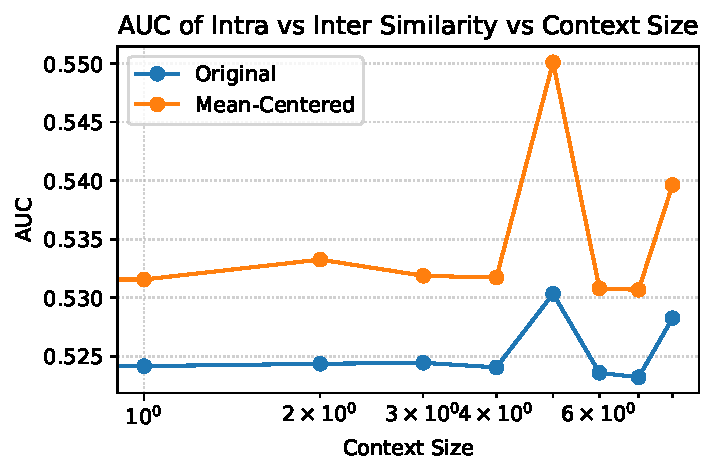
\includegraphics[width=\linewidth]{./figures/auc_vs_context_size.pdf}
				\caption{AUC of inter-class and intra-class pair similarities before and after applying CCR}
			\end{figure}
		\end{column}
	\end{columns}
\end{frame}

\begin{frame}
	\frametitle{Problem: Similarity Scale Varies by Dataset}
	\begin{columns}[c]
		\begin{column}{0.55\textwidth}
			\begin{itemize}
				\item Different datasets have different similarity distributions
				\item Some: tight clusters (most examples have $\sim$0.95)
				\item Others: spread distributions (similarities $\sim$0.5)
				      % \item Fixed temperature $\gamma=1$ fails across tasks
			\end{itemize}

			\vspace{0.5em}
			\heading{Impact on Classification}
			\begin{itemize}
				\item \textbf{High similarity:} Weights too uniform\\
				      $\rightarrow$ Averaging over irrelevant examples
				\item \textbf{Low similarity:} Weights too peaked\\
				      $\rightarrow$ Overfitting to noisy nearest neighbor
			\end{itemize}
		\end{column}
		\begin{column}{0.45\textwidth}
			\heading{Dynamic Kernel Weights} (Modified Eq.~\ref{eq:tarl-kernel-weights})
			\[
				w_i = \frac{\exp(\gamma \cdot \text{sim}(\vx_q, \vx_i))}{\sum_{j=1}^k \exp(\gamma \cdot \text{sim}(\vx_q, \vx_j))}
			\]
			\vspace{0.5em}
			\begin{itemize}
				\item High $\gamma$ $\rightarrow$ peaked weights (near-neighbor)
				\item Low $\gamma$ $\rightarrow$ uniform weights (averaging)
				\item But how do we know what $\gamma$ to use?
			\end{itemize}
		\end{column}
	\end{columns}
\end{frame}

\begin{frame}
	\frametitle{Solution: Temperature Calibration}
	\begin{columns}[c]
		\begin{column}{0.5\textwidth}
			\heading{Heuristic Approach}
			\begin{itemize}
				\item Set $\gamma$ based on maximum similarity:
				      \[
					      \hat{\gamma} = \frac{1}{\max(-\text{sim}(\vx_q, \vx_i))}
				      \]
				\item If closest example is near-duplicate:\\
				      $\hat{\gamma} \rightarrow \infty$ (nearest-neighbor)
				\item If all examples distant:\\
				      $\hat{\gamma}$ small (averaging)
			\end{itemize}
		\end{column}
		\begin{column}{0.5\textwidth}
			\begin{secondaryblock}{Limitation}
				Heuristic works reasonably but suboptimal across datasets
			\end{secondaryblock}
			\vspace{0.5em}
			Not good enough!
			\begin{itemize}
				\item Can we \textbf{learn} to predict optimal $\gamma$?
				\item Without gradient-based training on target task?
			\end{itemize}
		\end{column}
	\end{columns}
\end{frame}

\begin{frame}
	\frametitle{\textbf{mTaRL}: Meta-Learning $\gamma$ Calibration}
	\begin{columns}[c]
		\begin{column}{0.55\textwidth}
			\begin{enumerate}
				\item Define \textbf{oracle classifier}: uses optimal $\gamma$ per task
				      \begin{itemize}
					      \item Optimal $\gamma$ minimizes cross-entropy on true label
					      \item In practice, found via grid search over candidate $\gamma$ values
				      \end{itemize}
				\item Extract \textbf{meta-features} from support set:
				      \begin{itemize}
					      \item Mean/variance of similarities
					      \item Class imbalance statistics
					      \item Context-query embedding distances
				      \end{itemize}
				\item Train regression model to predict $\gamma$
			\end{enumerate}
			\vspace{0.5em}
			\heading{Training Cost}
			\begin{itemize}
				\item $<$ 1 hour on auxiliary datasets
				\item No GPU required
				\item Generalizes to new tasks without retraining
			\end{itemize}
		\end{column}
		\begin{column}{0.45\textwidth}
			\begin{figure}
				\centering
				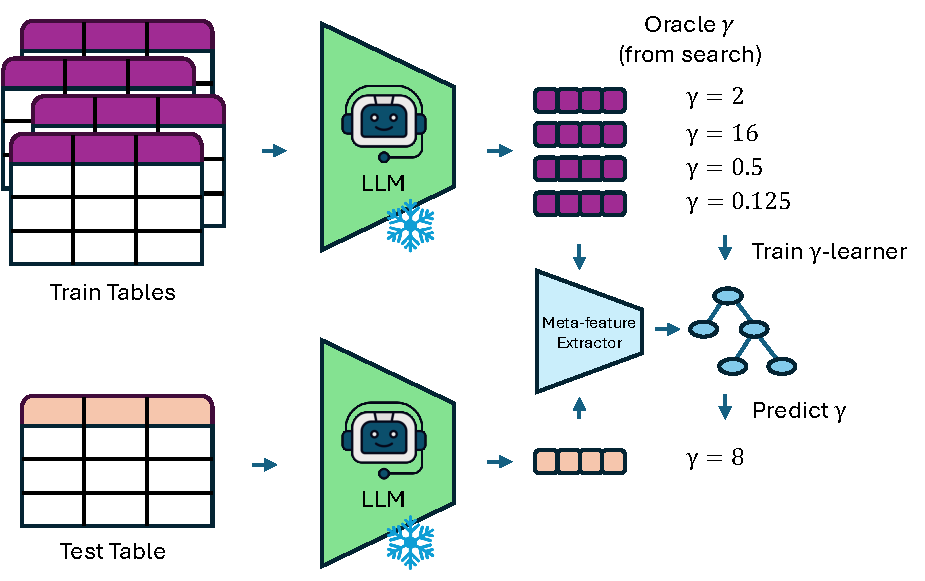
\includegraphics[width=\linewidth]{./figures/meta-training.pdf}
			\end{figure}
		\end{column}
	\end{columns}
\end{frame}

\begin{frame}
	\frametitle{The Complete \tarl{} Classifier}
	\heading{Algorithm Overview}
	\begin{enumerate}
		\item Serialize and embed support set $\{(\vx_i, y_i)\}_{i=1}^k$
		\item Serialize and embed query $\vx_q$
		\item Embed class labels $\{\vy_c\}_{c \in \mathcal{Y}}$
		\item Apply CCR to all embeddings
		\item Predict temperature $\gamma$ using meta-learned model
		\item Compute weighted sum of label embeddings:
		      \[
			      \bar{\vy}_q = \sum_{i=1}^k w_i \vy_{y_i}
		      \]
		\item Predict: $\hat{y}_q = \arg\max_{c} \text{sim}(\bar{\vy}_q, \vy_c)$
	\end{enumerate}
\end{frame}

\begin{frame}
	\frametitle{Experimental Setup}
	\begin{columns}[c]
		\begin{column}{0.5\textwidth}
			\heading{Datasets}
			\begin{itemize}
				\item \textbf{CARTE-CLF:} 60 diverse web tables with rich semantics~\cite{kasneciEnrichingTabularData2024}
				\item \textbf{TabArena:} 50 tables from UCI, Kaggle, OpenML~\cite{ericksonTabArenaLivingBenchmark2025}
			\end{itemize}
		\end{column}
		\begin{column}{0.5\textwidth}
			\heading{Baselines}
			\begin{itemize}
				\item XGBoost (classic ML)
				\item TabPFN (specialized tabular model)
				\item ConTextTab (LLM-based table model)
				\item TabuLa-8B (LLM fine-tuning + autoregressive)
			\end{itemize}
		\end{column}
	\end{columns}
\end{frame}

\begin{frame}
	\frametitle{Results: Performance on Semantic-Rich Datasets (CARTE-CLF)}
	\begin{columns}[c]
		\begin{column}{0.60\textwidth}
			\begin{figure}
				\centering
				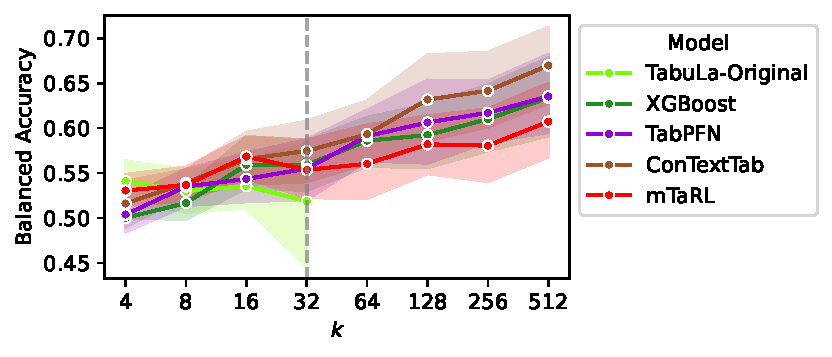
\includegraphics[width=\linewidth]{./figures/carte_cat-tabula_comparison-main.pdf}
			\end{figure}
		\end{column}
		\begin{column}{0.40\textwidth}
			\begin{table}
				\centering
				\begin{tabular}{lr}
					\toprule
					\textbf{Method}   & \textbf{Avg. Rank} \\
					\midrule
					ConTextTab        & \textbf{6.3295}    \\
					\textsc{mTaRL}    & \textit{6.4886}    \\
					XGBoost           & 6.8295             \\
					TabPFN            & 6.9318             \\
					TabuLa (Original) & 6.5114             \\
					\bottomrule
				\end{tabular}
				\caption{Avg. Rank at $k\leq 32$}
			\end{table}
			\begin{itemize}
				\item \textsc{mTaRL} achieves \textbf{2nd best rank}
				\item Competitive with ConTextTab, TabPFN
				\item Outperforms TabuLa-8B (autoregressive)
			\end{itemize}
		\end{column}
	\end{columns}
\end{frame}

% \begin{frame}
% 	\frametitle{Results: Computational Efficiency}
% 	\begin{columns}[c]
% 		\begin{column}{0.5\textwidth}
% 			\heading{Runtime Comparison (TabuLa-8B)}
% 			\begin{center}
% 				\begin{tabular}{lrr}
% 					\toprule
% 					$k$ & \textbf{TabuLa (s)} & \textbf{\tarl{} (s)} \\
% 					\midrule
% 					2   & 36,868              & 30 ($\times$1232)    \\
% 					4   & 37,519              & 42 ($\times$889)     \\
% 					8   & 34,785              & 67 ($\times$518)     \\
% 					16  & 30,370              & 118 ($\times$257)    \\
% 					32  & 21,456              & 223 ($\times$96)     \\
% 					\bottomrule
% 				\end{tabular}
% 			\end{center}
%
% 			\vspace{0.5em}
% 			\heading{Scaling}
% 			\begin{itemize}
% 				\item \tarl{}: \underline{Linear} in $k$ (embed each row once)
% 				\item Autoregressive: \underline{Quadratic} in $k$ (full context)
% 			\end{itemize}
% 		\end{column}
% 		\begin{column}{0.5\textwidth}
% 			\begin{figure}
% 				\centering
% 				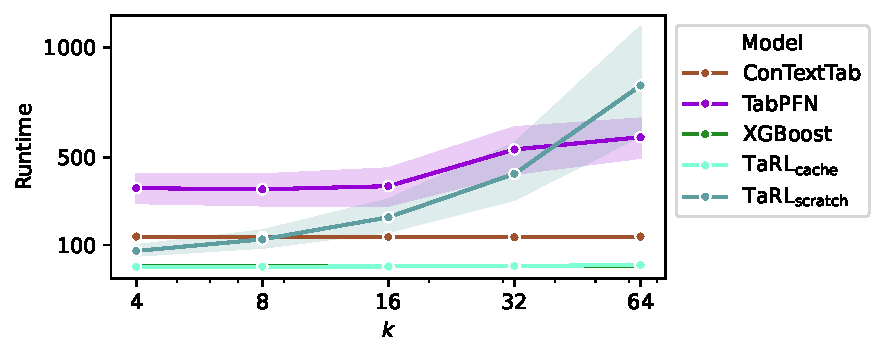
\includegraphics[width=\linewidth]{./figures/runtime-comparison.pdf}
% 			\end{figure}
% 			\vspace{0.5em}
% 			\begin{primaryblock}{Further Speedups}
% 				If embeddings pre-computed, inference is \textbf{near-instant} (only weight computation)
% 			\end{primaryblock}
% 		\end{column}
% 	\end{columns}
% \end{frame}

\begin{frame}
	\frametitle{Effect of Each Component in \tarl{}}
	\begin{columns}[c]
		\begin{column}{0.55\textwidth}
			\begin{figure}
				\centering
				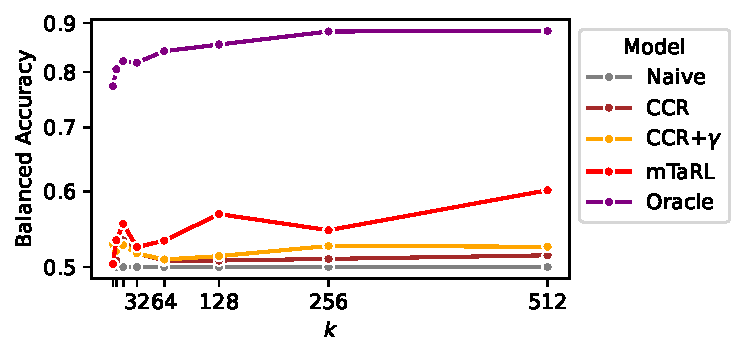
\includegraphics[width=0.9\linewidth]{./figures/carte_cat-lm_ablation.pdf}
			\end{figure}
		\end{column}
		\begin{column}{0.45\textwidth}
			\heading{Component Contributions}
			\begin{itemize}
				\item \textbf{Naive baseline:} Near random chance
				\item \textbf{+ CCR:} Significant boost
				      \begin{itemize}
					      \item Addresses anisotropy
				      \end{itemize}
				\item \textbf{+ Heuristic $\gamma$:} Further improvement
				      \begin{itemize}
					      \item Task-specific adaptation
				      \end{itemize}
				\item \textbf{+ Meta-learned $\gamma$:} Best practical
				      \begin{itemize}
					      \item Closes gap to oracle
				      \end{itemize}
			\end{itemize}
		\end{column}
	\end{columns}
	\vfill
	\begin{secondaryblock}{Oracle Gap}
		Significant room remains --- better $\gamma$ prediction could yield further gains
	\end{secondaryblock}
\end{frame}

\begin{frame}
	\frametitle{Summary}
	\vspace{1em}
	\begin{columns}[T]
		\begin{column}{0.55\textwidth}
			\heading{Contributions}
			\begin{itemize}
				\item Efficient representation extraction from \textbf{frozen LLMs} without fine-tuning
				\item Two key adaptations unlock embedding potential:
				      \begin{itemize}
					      \item \textbf{CCR:} Geometric correction for isotropy
					      \item \textbf{Temperature calibration:} Task-specific adaptation
				      \end{itemize}
				\item Competitive with SotA on \textbf{semantic-rich} tables
				\item \textbf{96--1232$\times$ speedup} over autoregressive
				\item Accepted to WebConf 2026
			\end{itemize}
		\end{column}
		\begin{column}{0.45\textwidth}
			\heading{Limitation/Future Work}
			\begin{itemize}
				\item Single-table classification
				\item Doesn't leverage \textbf{cross-table structure}
				\item Row-level embeddings lose column co-occurrence information
			\end{itemize}
		\end{column}
	\end{columns}
\end{frame}

\begin{frame}[allowframebreaks]
	\frametitle{References}
	\printbibliography
\end{frame}

\end{document}
